%%%%%%%%%%%%%%%%%%%%%%%%%%%%%%%%%%%%%%%%%%%%%%%%%%%%%%%
%% Bachelor's & Master's Thesis Template             %%
%% Copyleft by Artur M. Brodzki & Piotr Woźniak      %%
%% Faculty of Electronics and Information Technology %%
%% Warsaw University of Technology, 2019-2020        %%
%%%%%%%%%%%%%%%%%%%%%%%%%%%%%%%%%%%%%%%%%%%%%%%%%%%%%%%

\documentclass[
    left=2.5cm,         % Sadly, generic margin parameter
    right=2.5cm,        % doesnt't work, as it is
    top=2.5cm,          % superseded by more specific
    bottom=3cm,         % left...bottom parameters.
    bindingoffset=6mm,  % Optional binding offset.
    nohyphenation=false % You may turn off hyphenation, if don't like.
]{eiti/eiti-thesis}
\usepackage{float}
\langpol % Dla języka angielskiego mamy \langeng
\graphicspath{{img/}}             % Katalog z obrazkami.

\begin{document}

%--------------------------------------
% Strona tytułowa
%--------------------------------------
\MasterThesis % Dla pracy inżynierskiej mamy \EngineerThesis
\instytut{Informatyki i Automatyki Stosowanej}
\kierunek{Automatyka i Robotyka}
\specjalnosc{XXXXXX}
\title{
    Modelowanie i sterowanie rozmyte nieliniowego obiektu
}
\engtitle{ % Tytuł po angielsku do angielskiego streszczenia
    Unnecessarily long and complicated thesis' title \\
    difficult to read, understand and pronounce
}
\author{Maciej Kłos}
\album{270806}
\promotor{dr inż. Piotr Marusak}
\date{\the\year}
\maketitle

%--------------------------------------
% Spis treści
%--------------------------------------
\newpage
\tableofcontents

%--------------------------------------
% Rozdziały
%--------------------------------------
\cleardoublepage % Zaczynamy od nieparzystej strony
\pagestyle{headings}

\newpage % Rozdziały zaczynamy od nowej strony.
\section{Cel pracy}
Celem pracy jest zbadanie możliwości wykorzystania logiki rozmytej do procesu modelowania oraz do sterowania obiektami nieliniowymi. Na początek badana będzie jedna klasa obiektów nieliniowych - reaktory chemiczne. Celem jest zaproponowanie podejścia do procesu modelowania, który sprawdzałby się dla różnych obiektów tej kategorii. Uzyskany model, wykorzystujący logikę rozmytą, powinien dawać lepsze rezultaty pod względem wydajności, dokładności oraz prostoty zastosowania. Uzyskany model zostanie wykorzystany do zaprojektowania rozmytego regulatora nieliniowego obiektu.

     
\section{Opis reaktora polimeryzacji}
Do badań został wykorzystany reaktor polimeryzacji. Jest on schematycznie przedstawiony na rysunku \ref{fig:schemat_reaktor}.
\begin{figure}[H]
	\centering \includegraphics[width=0.8\linewidth]{schemat_reaktor.png}
	\caption{Schemat reaktora polimeryzacji}
	\label{fig:schemat_reaktor}
\end{figure}
Opisany jest on następującymi równaniami stanu:
\begin{equation}
\begin{split}
\dot{x}_1 &= - \left[Z_P\exp\left(\frac{-E_P}{RT}\right) + Z_{f_m}\exp\left(\frac{-E_{f_m}}{RT}\right)\right]x_1P_0(x_2, T) - \frac{Fx_1}{V} + \frac{FC_{m_{in}}}{V} \\
\dot{x}_2 &= - Z_I\exp\left(\frac{-E_I}{RT}\right)x_2 - \frac{Fx_2}{V} + \frac{f_IC_{I_{in}}}{V} \\
\dot{x}_3 &= \left[0.5Z_{T_C}\exp\left(\frac{-E_{T_C}}{RT}\right) + Z_{T_d}\exp\left(\frac{-E_{T_d}}{RT}\right)\right]P_0^2(x_2, T) + Z_{f_m} \exp\left(\frac{-E_{f_m}}{RT}\right) x_1P_0(x_2, T) - \frac{Fx_3}{V} \\
\dot{x}_4 &= M_m\left[Z_P\exp\left(\frac{-E_P}{RT}\right) + Z_{f_m}\exp\left(\frac{-E_{f_m}}{RT}\right)\right]x_1P_0(x_2, T) - \frac{Fx_4}{V}
\end{split}
\end{equation}
gdzie:
\begin{equation}
P_0(x_2, T) = \left[\frac{2f*x_2Z_I\exp(-E_I/RT)}{Z_{T_d}\exp(E_{T_d}/RT)+\exp(-E_{T_C}/RT)}\right]^{1/2}
\end{equation}
Poszczególne zmienne stanu mają następujące znaczenia:
\begin{itemize}
	\item $x_1 = C_m$
	\item $x_2 = C_I$
	\item $x_3 = D_0$
	\item $x_4 = D_I$
	\item $u = F_I$
	\item $y = \frac{D_I}{D_0}$
	\item $d = C_{m_{in}}$
\end{itemize}
Po podstawieniu parametrów reaktora otrzymujemy następujące uproszczone równania stanu:
\begin{equation}
\begin{split}
\dot{x}_1 &= -10x_1 - 2,4568x_1\sqrt{x_2} + 10d\\
\dot{x}_2 &= - 80u - 10,1022x_2\\
\dot{x}_3 &= 0,0024121x1\sqrt{x_2} + 0,112191x_2 - 10x_3 \\
\dot{x}_4 &= 245,978x_1\sqrt{x_2} - 10x_4 \\
y &= \frac{x_4}{x_3}
\end{split}
\end{equation}
Przedstawiony obiekt został zasymulowany w programie MATLAB za pomocą metedy Rungego-Kutty 4. rzędu z czasem próbkowania $T_s = 0,01h$.   
\section{Model statyczny obiektu}
Przyjęty został następujący punkt pracy:
\begin{itemize}
	\item $x_{1_0} = 5,50677$
	\item $x_{2_0} = 0,132906$
	\item $x_{3_0} = 0,0019752$
	\item $x_{4_0} = 49,3818$
	\item $u_0 = 0,016783$
	\item $y_0 = 25000,911$
	\item $d_0 = 6,0$
\end{itemize}
Zakres dopuszczalnych sterowań został przyjęty jako $ u \in (0.0016783; 0.067132)$Z tego punktu wykonano serię skoków co $\Delta u = 0,0034$ i po każdym z nich odczekiwano 150 iteracji. Wyniki przedstawione zostały na rysunku \ref{fig:statyka-odpowiedzi}.
\begin{figure}[!h]
	\centering 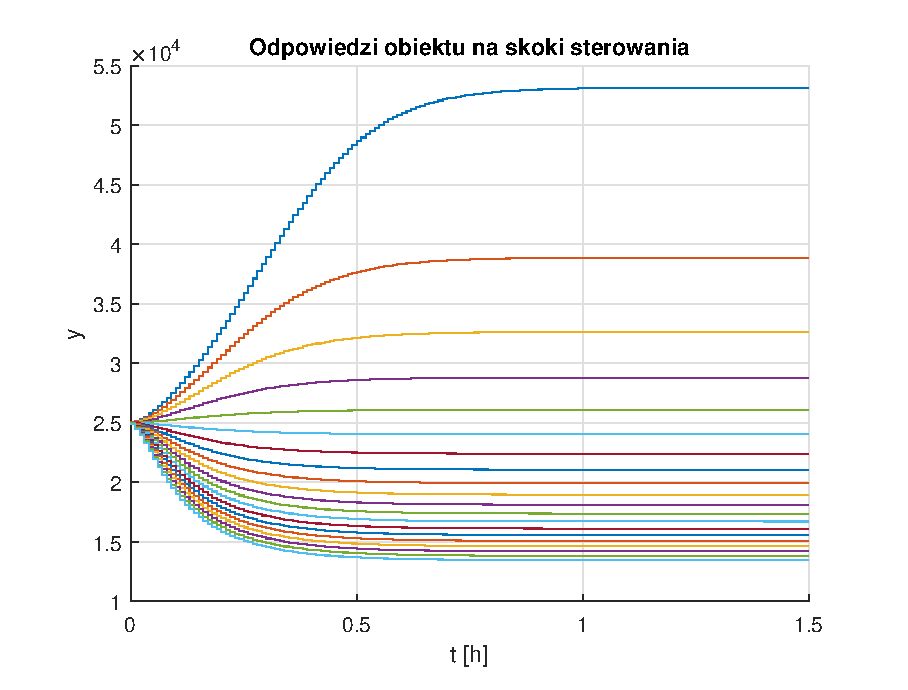
\includegraphics[width=0.8\linewidth]{statyka-odpowiedzi.eps}
	\caption{Odpowiedzi obiektu na skoki sterowania}
	\label{fig:statyka-odpowiedzi}
\end{figure}
Wartości z końca symulacji zostały zapisane do charakterystyki statycznej przedstawionej na rysunku \ref{fig:statyka-charakterystyka}.
\begin{figure}[!h]
	\centering \includegraphics[width=0.8\linewidth]{statyka-charakterystyka.eps}
	\caption{Charakterystyka statyczna obiektu}
	\label{fig:statyka-charakterystyka}
\end{figure}
Do modelowania charakterystyki użyto modelu Takagi-Sugeno o~czterech funkcjach przynależności przedstawionych na rysunku \ref{fig:mf}.
\begin{figure}[!h]
	\centering 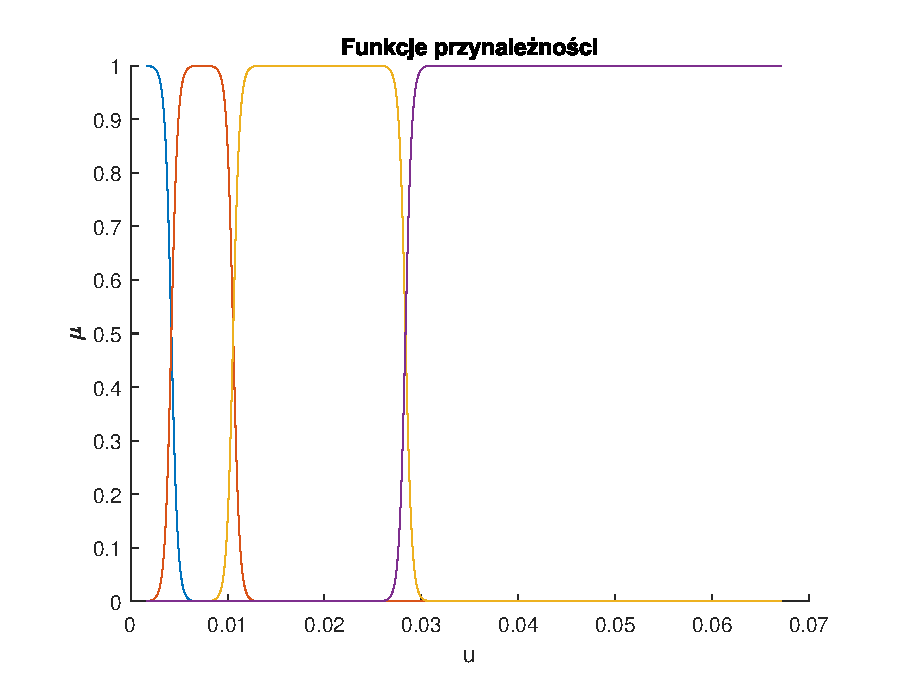
\includegraphics[width=0.8\linewidth]{mf.eps}
	\caption{Funkcje przynależności dla modelu statycznego obiektu}
	\label{fig:mf}
\end{figure}
\\Do każdej z nich przyporządkowany został model liniowy postaci:
\begin{equation}
y_{s_k}(u) = a_k\cdot u + b_k \qquad \textrm{gdzie } k = 1, 2, 3, 4
\end{equation}
Modele liniowe $y_{f_k}(u)$ uzyskano rozwiązując zadanie najmniejszych kwadratów na pewnym zakresie charakterystyki statycznej, zwiększając stopniowo ten zakres dopóki błąd średniokwadratowy pomiędzy modelem liniowym, a danymi nie przekroczył wartości progowej. Następnie zakres był przesuwany dalej i proces był powtarzany aż do osiągnięcia końcowej wartości $u$. Modele te przedstawione zostały na rysunku \ref{fig:modele-liniowe}.
\begin{figure}[!h]
	\centering 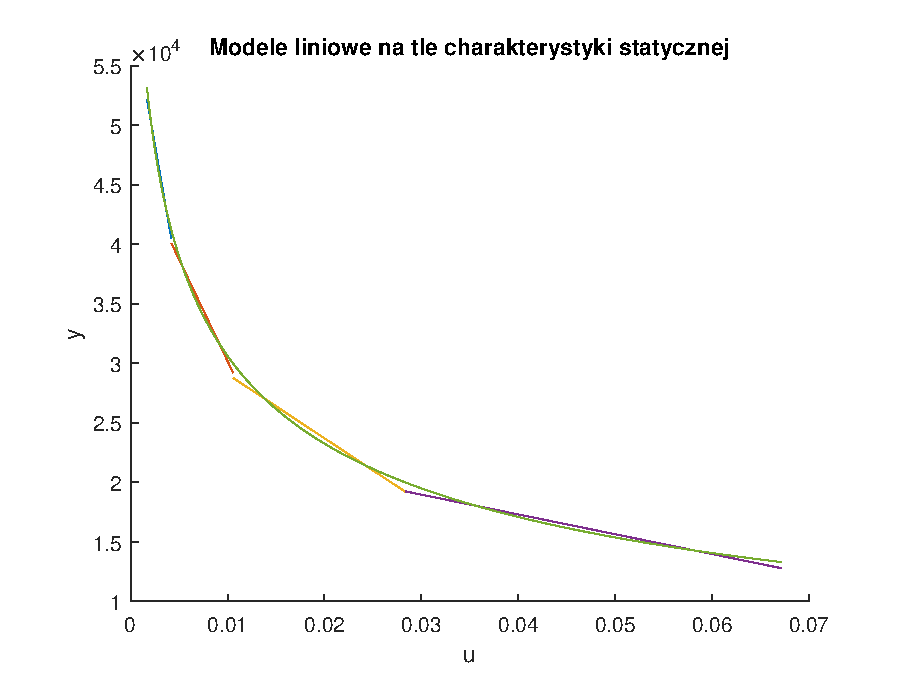
\includegraphics[width=0.8\linewidth]{modele-liniowe.eps}
	\caption{Funkcje przynależności dla modelu statycznego obiektu}
	\label{fig:modele-liniowe}
\end{figure}
Ostateczne wyjście modelu na tle charakterystyki statycznej przedstawiono na rysunku \ref{fig:statyka-model-rozmyty}.
\begin{figure}[!h]
	\centering 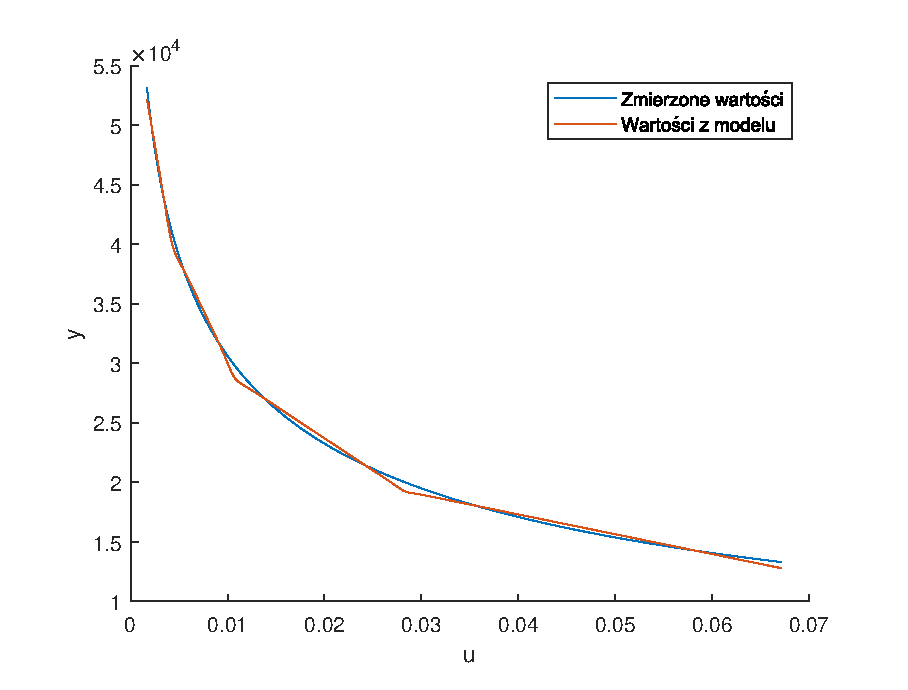
\includegraphics[width=0.8\linewidth]{statyka-model-rozmyty.eps}
	\caption{Wyjście rozmytego modelu statycznego}
	\label{fig:statyka-model-rozmyty}
\end{figure}
Błąd średniokwadratowy uzyskanego modelu wyniósł 1,29857e+05. Nie jest to bardzo dokładny model, jednakże bardziej skomplikowany model prowadziłby do zwiększenia nakładu obliczeniowego. Ponadto algorytmy regulacji całkują uchyb, przez co rozbieżności między modelem a obiektem będą kompensowane. 
\section{Model Hammersteina}
Aby zamodelować dynamikę obiektu zdecydowano się na użycie modelu Hammersteina, przedstawionego na rysunku \ref{fig:hammerstein}.
\begin{figure}[!h]
	\centering \includegraphics[width=1.0\linewidth]{hammerstein.png}
	\caption{Schemat modelu kaskadowego Hammersteina}
	\label{fig:hammerstein}
\end{figure}
W poprzednim punkcie wyznaczony został nieliniowy człon statyczny, teraz zajmiemy się liniowym członem dynamicznym. W tym celu na początek wyznaczono odpowiedź skokową z punktu pracy, zwiększając $u$ o 0,01. Wynik tego eksperymentu przedstawiono na rysunku \ref{fig:odpowiedz-skokowa}.
\begin{figure}[!h]
	\centering 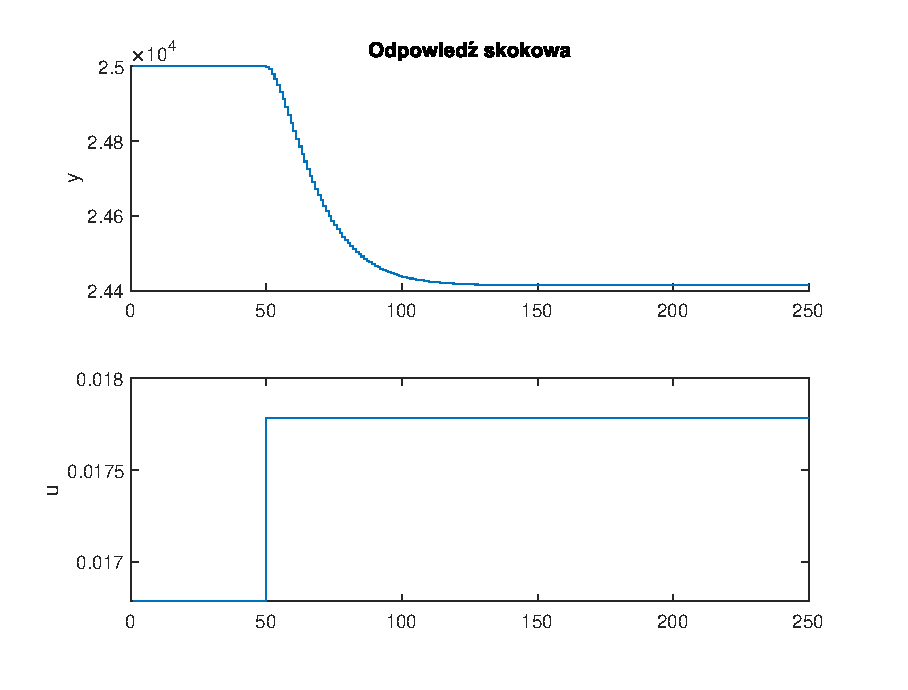
\includegraphics[width=0.8\linewidth]{odpowiedz-skokowa.eps}
	\caption{Odpowiedź skokowa obiektu}
	\label{fig:odpowiedz-skokowa}
\end{figure}
Przetestowano kilka rodzajów modelów, o różnych stopniach dynamiki, ostatecznie wybrano następujący:
\begin{equation}
\begin{split}
\hat{y}_d(k) = &a_1y(k-1) + a_2y(k-2)+a_3y(k-3)+a_4y(k-4)+ \\
+ &b_0u(k) +b_1u(k-1)+b_2u(k-2)+b_3u(k-3)+b_4u(k-4)
\end{split}
\end{equation}
Następnie poddano obróbce odpowiedź skokową, mianowicie znormalizowano skok sterowania oraz wyjście tak aby na końcu wynosiły 1. W takim przypadku wystarczy dynamikę modelu przeskalować przez nieliniowy człon statyczny otrzymując nieliniowy model dynamiczny. Po dobraniu wartości parametrów za pomocą metody najmniejszych kwadratów, przebieg wyjścia modelu przedstawiono na rysunku \ref{fig:model-dynamiczny}.
\begin{figure}[!h]
	\centering 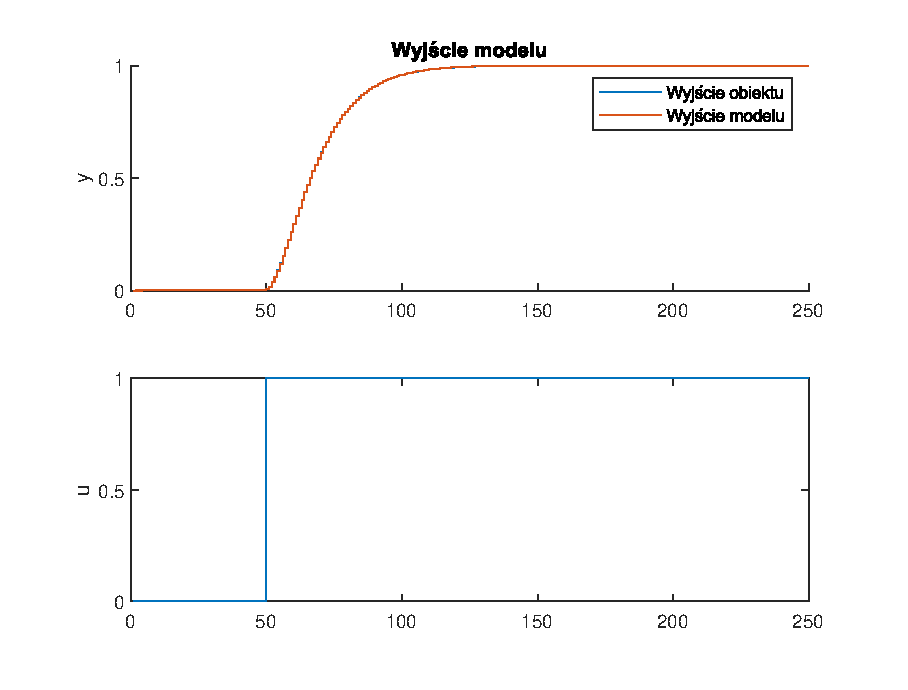
\includegraphics[width=0.8\linewidth]{model-dynamiczny.eps}
	\caption{Wyjście liniowego modelu dynamicznego}
	\label{fig:model-dynamiczny}
\end{figure}
Jak widać oba przebiegi się praktycznie pokrywają, błąd średniokwadratowy jest równy 4.1895e-08. Końcowy model będzie miał postać:
\begin{equation}
\begin{split}
\hat{y}(k) = &a_1y(k-1) + a_2y(k-2)+a_3y(k-3)+a_4y(k-4)+ \\
+ &\alpha(k) b_0u(k) +\alpha(k) b_1u(k-1)+\alpha(k) b_2u(k-2)+\alpha(k) b_3u(k-3)+\alpha(k) b_4u(k-4)
\end{split}
\end{equation}
gdzie
\begin{equation}
	\alpha(k) = \frac{\hat{y}_s(u(k))}{u(k)}
\end{equation}
Przebieg wyjściowy dla tego modelu przedstawiono na rysunku \ref{fig:przebieg-hammerstein}.
\begin{figure}[!h]
	\centering 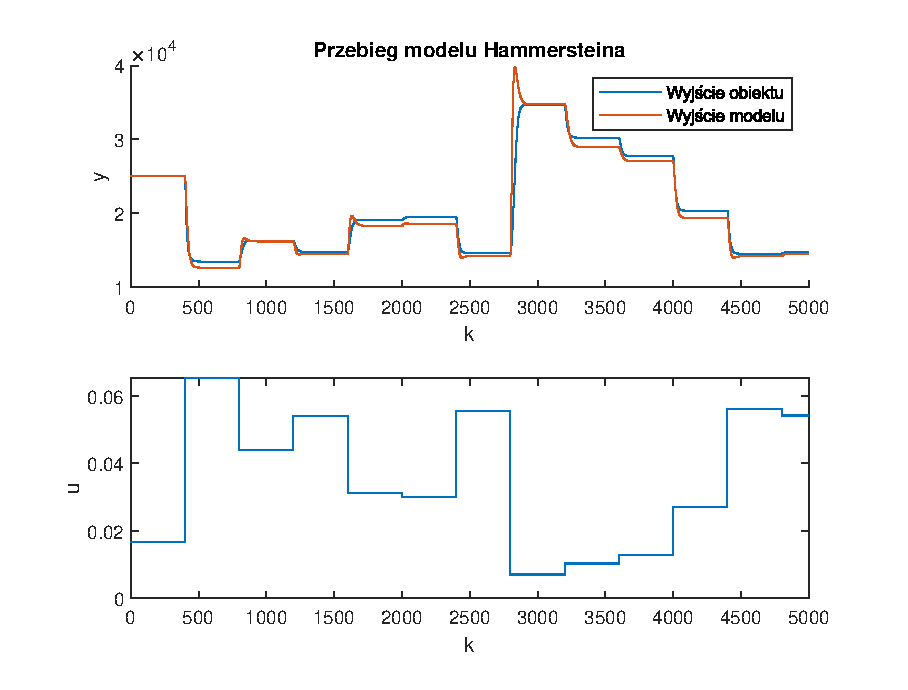
\includegraphics[width=0.8\linewidth]{przebieg-hammerstein.eps}
	\caption{Przebieg dla modelu Hammersteina}
	\label{fig:przebieg-hammerstein}
\end{figure}
Jak widać model w stanach ustalonych przyjmuje wartości statyczne wyliczone w poprzednim punkcie. Dynamika też jest w miarę dobrze odwzorowana, jednakże pojawiają się odchylenia w niektórych momentach. Może być to wina implementacji, co zostanie jeszcze zbadane w przyszłym semestrze. Błąd średniokwadratowy dla tego przebiegu był równy 6,4393e+08. 
\newpage
\section{Sterowanie obiektu}
\subsection{Klasyczny DMC}
Na początek zdecydowano się przetestować klasyczny algorytm DMC. W tym celu zebrano odpowiedź skokową w punkcie pracy. Została ona przedstawiona na rysunku \ref{fig:normalDMCs}.
\begin{figure}[!h]
	\centering 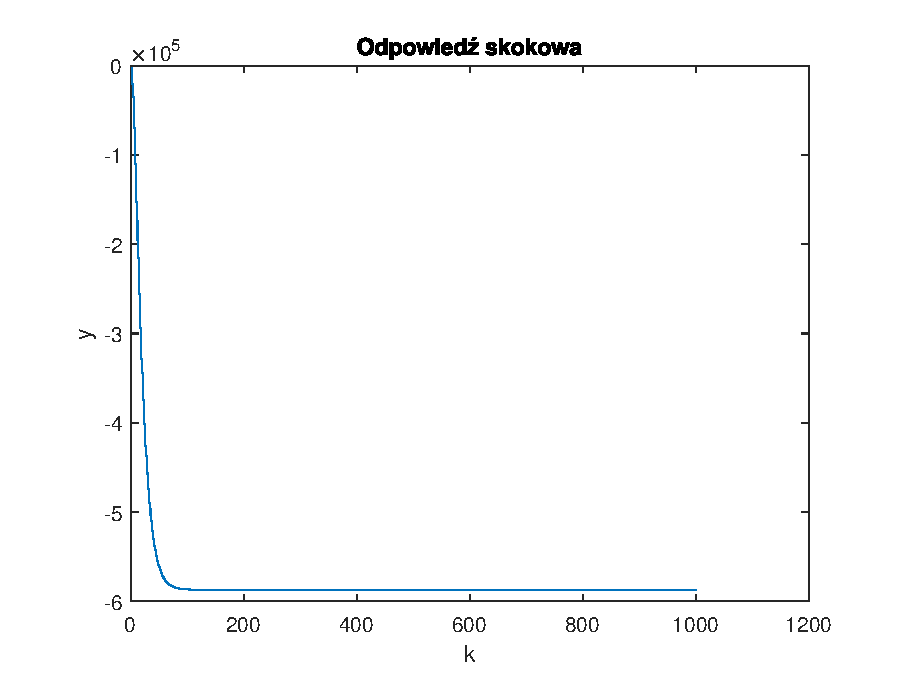
\includegraphics[width=0.8\linewidth]{normalDMCs.eps}
	\caption{Odpowiedź skokowa dla klasycznego algorytmu DMC}
	\label{fig:normalDMCs}
\end{figure}
Zaimplementowano algorytm DMC w wersji analitycznej. Przyjęto parametry regulatora $D =200$, $N= 200$, $N_U = 200$, $\lambda=1e+8$. Zostały one dobrane eksperymentalnie. Przebieg dla przykładowej trajektorii wartości zadanej został przedstawiony na rysunku \ref{fig:normalDMC}.
\begin{figure}[!h]
	\centering 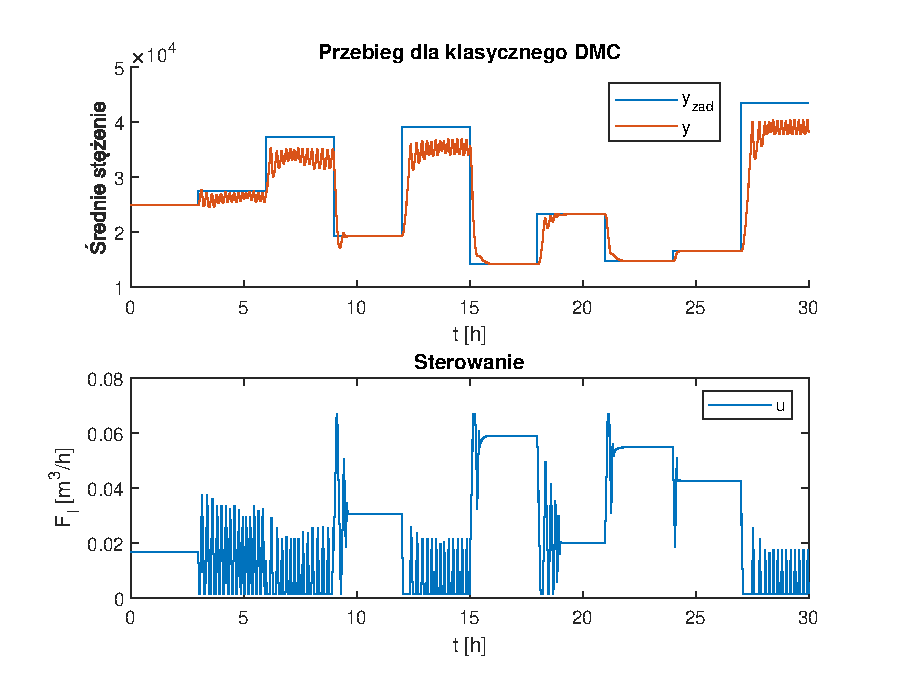
\includegraphics[width=0.8\linewidth]{normalDMC.eps}
	\caption{Przebieg dla klasycznego algorytmu DMC}
	\label{fig:normalDMC}
\end{figure}

Jak widać regulator nie radzi sobie dobrze, występują duże oscylacje, oraz uchyby ustalone. Warto też zauważyć że parametr $\lambda$ jest bardzo duży. Błąd dla tego przebiegu wyniósł 5,5095e+10. Eksperyment ten pokazuje że w przypadku badanego reaktora istnieje potrzeba zastosowania algorytmu regulacji opartego na modelu nieliniowym.

\subsection{DMC-SL}
Do zaprojektowania regulatora DMC-SL w wersji analitycznej wykorzystano odpowiedź skokową modelu dynamicznego z poprzedniego punktu. Została ona przedstawiona na rysunku \ref{fig:DMC-SLs}.
\begin{figure}[H]
	\centering 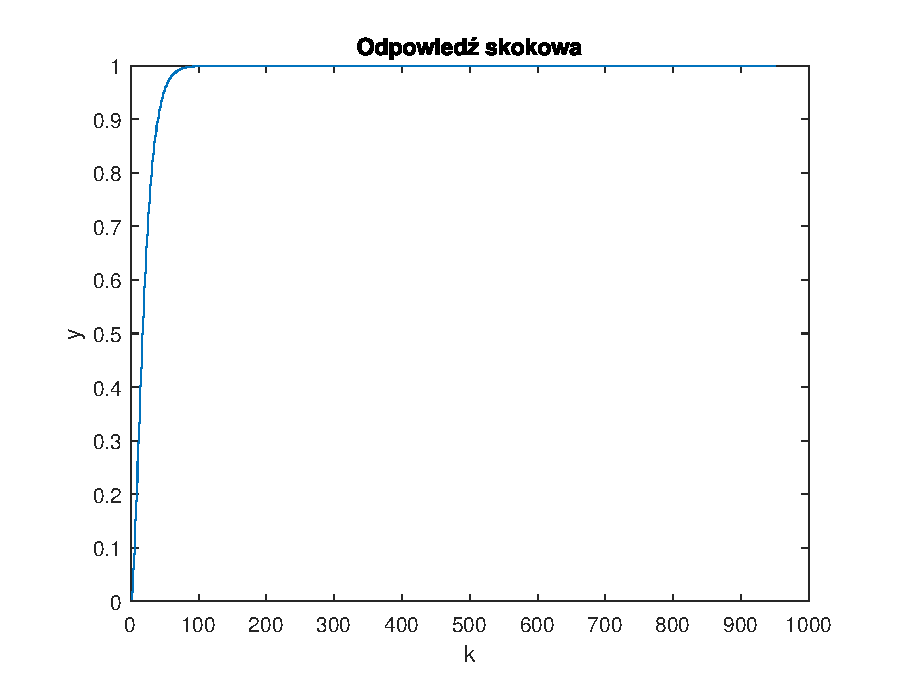
\includegraphics[width=0.8\linewidth]{DMC-SLs.eps}
	\caption{Odpowiedź skokowa dla algorytmu DMC-SL}
	\label{fig:DMC-SLs}
\end{figure}
W każdej iteracji jest ona przemnażana przez współczynnik $\alpha(k)$, co daje odpowiedź skokową w danej chwili. Wszystkie parametry regulatora są takie same jak w poprzednim podpunkcie. Przebieg dla tego regulatora został przedstawiony na rysunku \ref{fig:DMC-SL}.
\begin{figure}[H]
	\centering 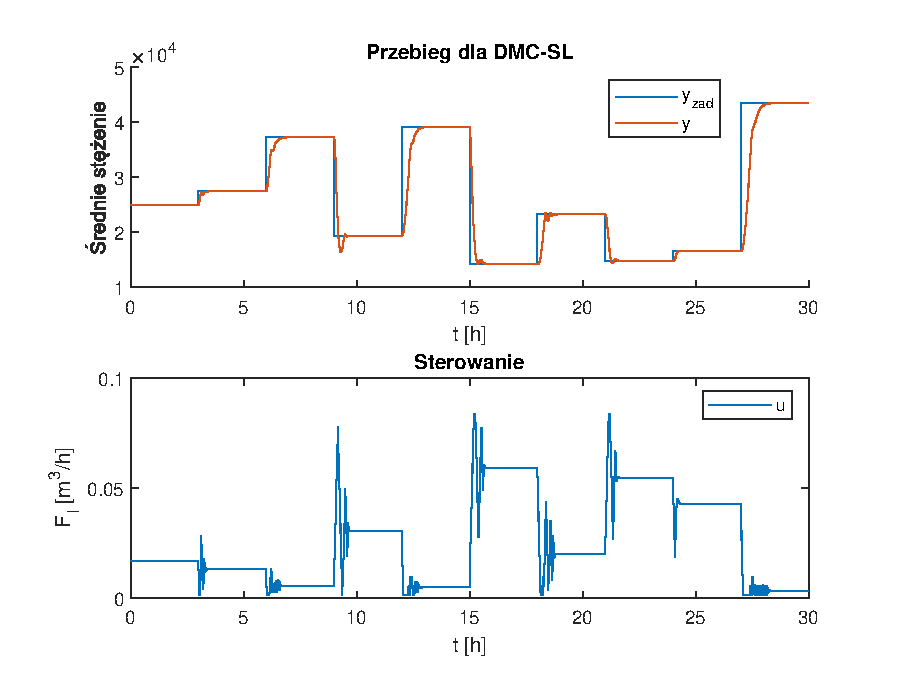
\includegraphics[width=0.8\linewidth]{DMC-SL.eps}
	\caption{Przebieg dla algorytmu DMC-SL}
	\label{fig:DMC-SL}
\end{figure}
Jak widać przebieg jest znacznie bardziej stabilny, nie występują też żadne uchyby ustalone. Błąd też uległ poprawie, był równy 4.0812e+10. Wykorzystanie zaprojektowanego modelu daje znaczne korzyści w przypadku obiektu nieliniowego z którym mamy tutaj do czynienia. Można dostroić parametry tego regulatora. Na przykład warto rozważyć zmniejszenie współczynnika $\lambda$, co powinno zwiększyć szybkość regulacji, kosztem bardziej gwałtownego przebiegu sterowania i szansy na pojawienie się oscylacji. 

\newpage % Rozdziały zaczynamy od nowej strony

%--------------------------------------------
% Spisy (opcjonalne)
%--------------------------------------------
\newpage
\pagestyle{plain}

% Wykaz symboli i skrótów.
% Pamiętaj, żeby posortować symbole alfabetycznie
% we własnym zakresie. Ponieważ mało kto używa takiego wykazu,
% uznałem, że robienie automatycznie sortowanej listy
% na poziomie LaTeXa to za duży overkill.
% Makro \acronymlist generuje właściwy tytuł sekcji,
% w zależności od języka.
% Makro \acronym dodaje skrót/symbol do listy,
% zapewniając podstawowe formatowanie.
% //AB
\vspace{0.8cm}
\listoffigurestoc     % Spis rysunków.
\vspace{1cm}          % vertical space


% Używając powyższych spisów jako szablonu,
% możesz tu dodać swój własny wykaz bądź listę,
% np. spis algorytmów.

\end{document} % Dobranoc.
